\documentclass{beamer}

\mode<presentation>
{
  \usetheme{EEng}
  \setbeamercovered{transparent}
  \setbeamercolor{background canvas}{bg=black!0}
}

\usepackage{enumerate}
\usepackage{array}
\usepackage{pifont} % for \cross symbol newcommand
\usepackage{graphics}
\usepackage{graphicx}
\usepackage{ucs}
\usepackage[utf8x]{inputenc}
\usepackage[english]{babel}
\usepackage{amsmath, amsthm, amssymb}
\usepackage[caption=false,font=footnotesize]{subfig}
\usepackage{amsmath}
\usepackage{amsfonts}
\usepackage{url}
\usepackage{listings}
\usepackage{color}

\newcommand{\checkK}{\color{green}\checkmark}
\newcommand{\cross}{\color{red}\hspace{-3pt}\ding{55}}
\newcommand{\bigexclaim}{\color{Dandelion}$\bigtriangleup$\hspace{-5.6pt}!}
\lstdefinelanguage{codeTTN}
{
        basicstyle=\ttfamily\tiny,
        sensitive=true,
        showstringspaces=false,
        numberblanklines=true,
        showspaces=false,
        breaklines=true,
        showtabs=false,
		numbers=left,
		numberstyle=\tiny,
		xleftmargin=15pt,
}
\lstnewenvironment{code}{\lstset{language=codeTTN}}{}

\title{Automatic Test Generation for Space}
\author{Ulisses Costa \and Daniela da Cruz \and Pedro Rangel Henriques}
\institute{SLATE'12 - Symposium on Languages, Applications and Technologies}
\date{\today}

\begin{document}
\begin{frame}
   \titlepage
\end{frame}

\begin{frame}\frametitle{Context}
\begin{block}{Problem}
VST (Visionspace Technologies) provides services related to testing for ESA and wants to automate
the test generation for the Operational Simulator platform.
\end{block}

This presentation appears in the context of a master's thesis that aims at:
\begin{itemize}
\item Generate automatically tests for the \textit{Operational Simulator}
\item Generate unit tests for the \textit{Operational Simulator} language -- C++
\item Parametrize the size of the generated data structures and be able to configure other attributes
\end{itemize}
\end{frame}

\begin{frame}\frametitle{Motivation}
To:
\begin{itemize}
\item Extract UML and OCL from the existing code
\item Extract tests from the existing code
\end{itemize}
\end{frame}

\begin{frame}\frametitle{OCL Inference}
OCL is a language used to describe logic properties about UML models, typically in the form of invariants.

The first step is to extract interesting invariants from the code and match them with requirements.
\begin{itemize}
\item Generate UML diagrams from the existing code (easy)
\item Infer code invariants (hard)
\item Relate the discovered invariants with the UML diagrams
\item Relate the discovered diagrams with requirements
\end{itemize}
\end{frame}

\begin{frame}\frametitle{White vs. Black Box Testing}
\begin{block}{Types of tests regarding the knowledge about the code}
\begin{description}
\item[White Box], there is knowledge about the code, and this is used to perform the test generation.
\item[Black Box], there is only knowledge about the requirements and about how each component should behave.
\end{description}
\end{block}
\end{frame}

\begin{frame}\frametitle{Approaches 1/2}
\begin{description}
\item[Specification-based Generation Testing], \textit{aka Model Based Testing} consists in testing a program based on the program specification or on the program model.
Test cases can be generated from the specification, without consider the code.
\end{description}
\end{frame}

\begin{frame}\frametitle{Approaches 2/2}
\begin{description}
\item[Constraint-based Generation Testing], can be used to select test cases that meet some variable restrictions.
When combined with symbolic execution, gathers restrictions along the different paths in the \textit{CFG}.
It is possible to solve these restrictions and generate test cases.
\end{description}
\end{frame}

\begin{frame}\frametitle{Current state}
By now, we studied different approaches and tools, the more important to our goal are:
\begin{itemize}
\item Korat, is a mature framework to automatically construct complex structures for JAVA
\item Pex is a \textit{White-box testing framework} from Microsoft tool that tries to give total code coverage
\end{itemize}
\end{frame}

\begin{frame}[fragile] \frametitle{Studied Tools - Pex}
\begin{code}
public class Program {
  public static int BSearch(int x, int n) {
    return BinarySearch(x, 0, n);
  }
  static int BinarySearch(int x, int lo, int hi) {
    while (lo < hi) {
      int mid = (lo+hi)/2;
      Debug.Assert(mid >= lo && mid < hi);
      if (x < mid) { hi = mid; } else { lo = mid+1; }
    }
    return lo;
  }
}
\end{code}

{\tiny \begin{tabular}{|c|c|c|c|c|}\hline
Result & x & n & result & Output/Exception \\\hline
\checkK & 0 & 0 & 0      & \\\hline
\checkK & 0 & 1 & 1      & \\\hline
\checkK & 0 & 3 & 1      & \\\hline
\cross & 1073741888 & 1719676992 & & TraceAssertionException \\\hline
\checkK & 1 & 6 & 2      & \\\hline
\checkK & 50 & 96 & 51      &\\\hline
\end{tabular}
}
\end{frame}

\def\t#1#2#3#4{\langle#1 \ #2 : #3 \ : #4 \ \rangle}
\def\d#1#2#3{\langle#1 \ #2 :: #3 \ \rangle}
\newcommand{\subseteqL}{\mathbin{\subseteq\mkern-4mu\subseteq}}
\newcommand{\inL}{\mathbin{\in\mkern-4mu\in}}

\begin{frame}[fragile]\frametitle{Studied Tools - Korat}
\begin{code}
public class LinkedList<T> {
  public static class LinkedListElement<T> {
    public T Data;
    public LinkedListElement<T> Prev;
    public LinkedListElement<T> Next;
  }
  private LinkedListElement<T> Head;
  private LinkedListElement<T> Tail;
  private int size; 
}
\end{code}
$LinkedList$ class invariants (circular doubly linked list):
{\tiny
\begin{eqnarray}
\t \forall {l} {l \in LinkedList} {Head(l) \equiv null \vee Tail(l) \equiv null \Leftrightarrow size(l) \equiv 0}\\
\t \forall {l} {l \in LinkedList} {Tail(l).Next \equiv null}\\
\t \forall {l} {l \in LinkedList} {Head(l).Prev \equiv null}\\
\t \forall {l} {l \in LinkedList} {size(l) \equiv 1 \Leftrightarrow Head(l) \equiv Tail(l)}\\
\t \forall {l} {l \in LinkedList} {\t \forall {e_1,e_2} {\{e_1,e_2\} \subseteqL l} {\t \exists {e} {e \inL l} {e_1.Next \equiv e \wedge e_2.Prev \equiv e}}\label{eq:linked}}\\
\t \forall {l} {l \in LinkedList} {\t \forall {e_1,e_2} {\{e_1,e_2\} \subseteqL l} {e_1 \equiv e_2 \Rightarrow i(e_1) \equiv i(e_2)}\label{eq:uniq}}
\end{eqnarray}
}
\end{frame}

\begin{frame}[fragile]\frametitle{Studied Tools - Pex - $LinkedList$}
\begin{figure}[!ht]
\centerline{
\subfloat[$LinkedList$ instance generated by Pex to test the method $Remove$]{
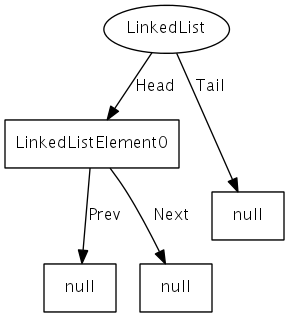
\includegraphics[width=.3\textwidth]{img/pex1}
}
\hfil
\subfloat[$LinkedList$ instance generated by Pex to test the method $Find$]{
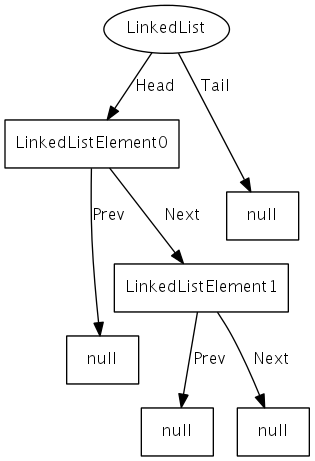
\includegraphics[width=.3\textwidth]{img/pex2}
\label{fig:pexinst2}}}
\caption{Examples of instances generated by Pex to the $LinkedList$ class.}
\label{fig:pexG}
\end{figure}
\end{frame}

\begin{frame}[fragile]\frametitle{Studied Tools - Korat - $LinkedList$}
\begin{figure}[!ht]
\centerline{
\subfloat[$LinkedList$ instance with $2$ elements]{
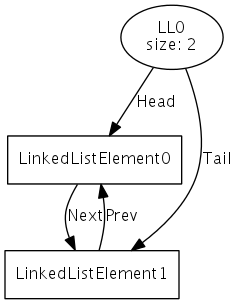
\includegraphics[width=.2\textwidth]{img/ll1}
}
\hfil
\subfloat[$LinkedList$ instance with $5$ elements]{
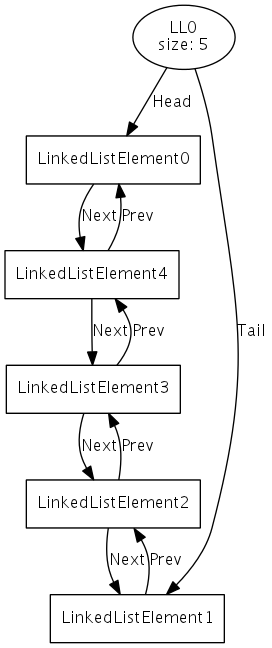
\includegraphics[width=.2\textwidth]{img/ll2}
}}
\end{figure}
\end{frame}

\begin{frame}[fragile]\frametitle{Studied Tools - Summary}
\begin{block}{Summary}
Pex uses static analysis and is very efficient in discovering all the possible execution paths in C\# methods.
Pex can also be used to generate classes testcases, but the generated instances does not keep the invariants of data structures.\\

On the other hand, Korat is the ideal tool to generate data structures that meet the invariants.
\end{block}
\end{frame}

\begin{frame} \frametitle{Conclusion and Future work}
\begin{itemize}
\item Pex has proved to be a powerful tool regarding full coverage.
\item Korat is a very useful tool to generate complex data structures.
\end{itemize}
A mix between the static analysis of Pex with Korat's capability to generate useful data structures is the path we will follow.\\

The study of pre- pos conditions inference using static analysis [Moy 2009] will be useful to infer OCL rules.
\end{frame}

\begin{frame}[fragile] \frametitle{Korat $repOK$ method for $LinkedList$}
\begin{code}
public boolean repOK() {
  if(Head == null || Tail == null)
    return size == 0;
  if(size == 1) return Head == Tail;
  if(Head.Prev != null) return false;
  if(Tail.Next != null) return false;
  LinkedListElement<T> last = Head;
  Set visited = new HashSet();
  LinkedList workList = new LinkedList();
  visited.add(Head);
  workList.add(Head);
  while (!workList.isEmpty()) {
    LinkedListElement<T> current = (LinkedListElement<T>) workList.removeFirst();
    if (current.Next != null) {
      if (!visited.add(current.Next))
	    return false;
      workList.add(current.Next);
      if(current.Next.Prev != current) return false;
      last = current.Next;
    }
  }
  if(last != Tail)
    return false;
  return (visited.size() == size);
}
\end{code}
\end{frame}

\end{document}

